\documentclass[a4paper,10pt]{article}
\usepackage{graphicx}
\usepackage[ansinew]{inputenc}
\usepackage[spanish]{babel}
\usepackage{listings}
\inputencoding{latin1}

\title{		\textbf{Trabajo Pr\'{a}ctico 0: \\
			Infraestructura b\'{a}sica
			}}

\author{	Fabrizio Cozza, \textit{Padr\'{o}n Nro. 97.402}                     \\
            \texttt{ fabrizio.cozza@gmail.com }                                              \\[2.5ex]
            Kevin Cajachu\'{a}n, \textit{Padr\'{o}n Nro. 98.725}                     \\
            \texttt{ kevincajachuan@hotmail.com }                                              \\[2.5ex]
            Luciano Giannotti, \textit{Padr\'{o}n Nro. 97.215}                     \\
            \texttt{luciano\_giannotti@hotmail.com.ar}                                              \\[3.5ex]
	 \newline
            \normalsize{1er. Cuatrimestre de 2018}                                      \\
            \normalsize{66.20 Organizaci\'{o}n de Computadoras  $-$ Pr\'{a}ctica Viernes}  \\
            \normalsize{Facultad de Ingenier\'{i}a, Universidad de Buenos Aires}            \\
       }
\date{}


\begin{document}
\maketitle
\thispagestyle{empty}   % quita el n�mero en la primer p�gina


\section{Objetivos}

Este Trabajo Pr\'{a}ctico tiene el fin de ayudarnos a familiarizarnos con las herramientas de software que utilizaremos posteriormente en otros trabajos, como es el emulador \textbf{gxemul} para correr programas sobre una maquina MIPS con el Sitema Operativo NetBSD.


\section{Programa}

El software de este trabajo esta escrito en lenguaje C y permite dibujar \textbf{Julia Sets} o \textbf{Conjuntos de Julia} segun los par\'{a}metros que le pasamos por l\'{i}nea de comando.
Estos parámetros son la region del plano complejo: delimitada por un centro, un ancho y un alto; una semilla que afectara el calculo para c\'{a}da pixel; la resoluci\'{o}n y la salida ya sea por pantalla o por archivo.
El formato a usar es  PGM o \textit{portable gray format}, que resulta \'{u}til para describir im\'{a}genes digitales en escala de grises.


\section{Implementaci\'{o}n}

Una vez recibidos los par\'{a}metros, para dibujar el Julia Set el programa obtiene de cada p\'{i}xel de la ventana a un punto en el plano complejo.
A ese punto se lo eleva al cuadrado y le suma la semilla mencionada en la secci\'{o}n anterior. Esto se repite hasta que el valor absoluto del resultado sea menor a 2, en cuyo caso se toma la cantidad de iteraciones y se imprime en el archivo PGM, representando el nivel de blanco de ese pi\'{i}xel.


\section{C\'{o}digo}

En esta secci\'{o}n colocaremos el ci\'{o}digo fuente del programa en lenguaje C.


\section{Pruebas}

Para las pruebas compilamos el programa con gcc de la siguiente manera:

\begin{lstlisting}[frame=single]
$gcc main.c -o tp0
\end{lstlisting}

Ya que las pruebas son sobre las imágenes, las vamos a realizar a ojo.

\subsection{Caso con los valores por defecto}
Se obtiene una imagen como la primera figura del enunciado:

\begin{lstlisting}[frame=single]
$.\tp0 -o uno.pgm
\end{lstlisting}

\begin{figure}[!htp]
\begin{center}
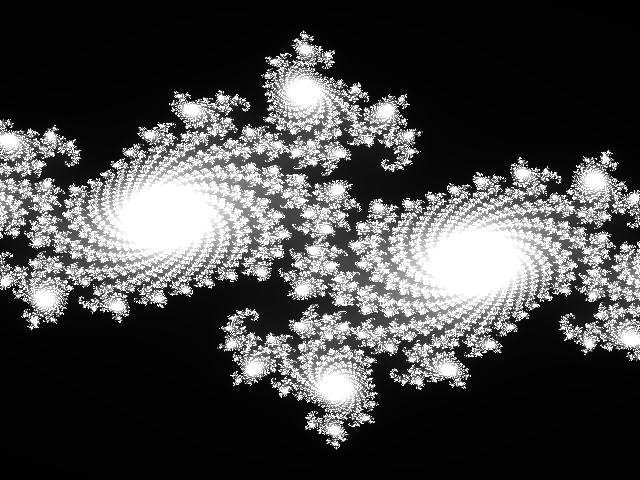
\includegraphics[width=0.5\textwidth]{uno.png}
\caption{} \label{}
\end{center}
\end{figure}

\subsection{Caso de imagen con zoom y otro centro}
Se obtiene una imagen como la segunda figura del enunciado:

\begin{lstlisting}[frame=single]
$ .\tp0 -c 0.282-0.007i -w 0.005 -H 0.005 -o dos.pgm
\end{lstlisting}

\begin{figure}[!htp]
\begin{center}
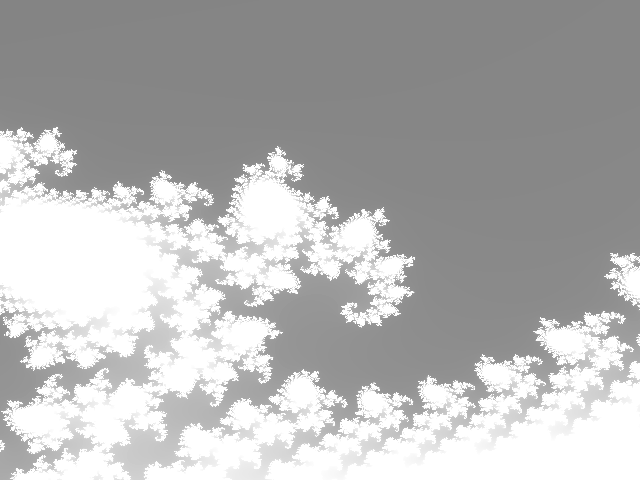
\includegraphics[width=0.5\textwidth]{dos.png}
\caption{} \label{}
\end{center}
\end{figure}

\begin{thebibliography}{99}

\bibitem{INT06} Intel Technology \& Research, ``Hyper-Threading Technology,'' 2006, http://www.intel.com/technology/hyperthread/.

\bibitem{HEN00} J. L. Hennessy and D. A. Patterson, ``Computer Architecture. A Quantitative
Approach,'' 3ra Edici�n, Morgan Kaufmann Publishers, 2000.

\bibitem{LAR92} J. Larus and T. Ball, ``Rewriting Executable Files to Mesure Program Behavior,'' Tech. Report 1083, Univ. of Wisconsin, 1992.

\end{thebibliography}

\end{document}
